\documentclass[12pt,x11names]{article}
\input{preamble}


\newgeometry{margin=2cm}

\pagestyle{fancy}
\fancyhf{}

\rhead{Nørre Gymnasium\\
1.m
}
\cfoot{Side \thepage \hspace{1pt} af \pageref{LastPage}}

%Husk at rette modul og dato!
\lhead{Matematik B\\
Årsprøve
}
\chead{ %25/3/2022
}

\begin{document}

%
\includepdf[pages=-]{Forsider/aarsprove_1v.pdf}
\savegeometry{art}

\begin{titlepage}
\newgeometry{margin=0pt}

\begin{minipage}{0.27\textwidth}

\begin{tikzpicture}[overlay]
\fill[top color = NorregGroen!40, bottom color = NorregGroen] (6,10) rectangle (-10,-30);
\end{tikzpicture}
\end{minipage}
\begin{minipage}{0.73\textwidth}
\begin{center}
\phantom{h} \vspace{1cm}\\
\hspace{4cm}

\includegraphics[scale = 1]{Billeder/Norreg.png} \\
\phantom{h} \vspace{5cm}\\
\Huge 1v Ma\\
Årsprøve \\
\large 25. maj 2022
\end{center}
\end{minipage}
\end{titlepage}
\loadgeometry{art}

%Udfyld afsnit herunder og lav til egen Latex-fil

%Kopier følgende til overskrift:

%\begin{center}
%\Huge
%Aflevering 1
%\end{center}
%\section*{Opgave 1}
%\stepcounter{section}
\section*{Krav til formidling af din besvarelse}
Ud for hvert delspørgsmål i opgaverne er angivet det antal point, hvormed besvarelsen af spørgsmålet indgår i den samlede bedømmelse. Der gives i alt 160 point.

Ved bedømmelse af helhedsindtrykket af besvarelsen af de enkelte opgaver lægges særlig vægt på følgende fire punkter:
\begin{itemize}
\item[$\cdot$] \textbf{Redegørelse og dokumentation for metode} \\
Besvarelsen skal indeholde en redegørelse for den anvendte løsningsstragegi med dokumentation i form af et passende antal mellemregninger \textit{eller} matematiske forklaringer på metoden, når et matematisk værktøjsprogram anvendes.
\item[$\cdot$] \textbf{Figurer, grafer og andre illustrationer} \\
Besvarelsen skal indeholde hensigtsmæssig brug af figurer, grafer og andre illustrationer, og der skal være tydelige henvisninger til brug af disse i den forklarende tekst.
\item[$\cdot$] \textbf{Notation og layout}\\
Besvarelsen skal i overensstemmelse med god matematisk skik opstilles med hensigtsmæssig brug af symbolsprog, og med en redegørelse for den matematiske notation, der indføres og anvendes, og som ikke kan henføres stil standardviden.
\item[$\cdot$] \textbf{Formidling og forklaring}\\
Besvarelsen af rene matematikopgaver skal indeholde en angivelse af givne oplysninger og korte forklaringer knyttet til den anvendte løsningsstrategi beskrevet med brug af almindelig matematisk notation. 

Besvarelsen af opgaver, der omhandler matematiske modeller, skal indeholde en kort præsentation af modellens kontekst, herunder betydning af modellens parametre. De enkelte delspørgsmål skal afsluttes med en præcis konklusion præsenteret i et klart sprog i relation til konteksten.
\end{itemize}

\newpage

\begin{center}
\Huge
Delprøve uden hjælpemidler (9:00 - 10:00)
\end{center}

\begin{opgavetekst}{Opgave 1}
\end{opgavetekst}
\begin{delopgave}{10 point}{1}
		Reducér udtrykket
		\begin{align*}
			a^2+2ab-(a+b)^2.
		\end{align*}	
\end{delopgave}
\begin{opgavetekst}{Opgave 2}
Løs følgende ligninger:
\end{opgavetekst}
\begin{delopgave}{5 point}{1}
	$6x-12=30$
\end{delopgave}
\begin{delopgave}{10 point}{2}
	$x^2-6x+5=0$
\end{delopgave}

\begin{opgavetekst}{Opgave 3}
Udviklingen i salget af teaterbilletter i Danmark kan tilnærmelsesvist beskrives ved modellen $f$ med forskriften
\begin{align*}
f(x) = 2.68\cdot 0.992^x,
\end{align*}
hvor $x$ er antal år siden år $1982$ og $f$ beskriver antallet af årligt solgte billetter i mio. 
\end{opgavetekst}
\begin{delopgave}{10 point}{1}
Hvad fortæller tallene $2.68$ og $0.992$ om det årlige antal solgte teaterbilletter?
\end{delopgave}

\begin{opgavetekst}{Opgave 4}
På Fig. \ref{fig:poly} ses parablen for et andengradspolynomium $f$ med forskriften
\begin{align*}
f(x) = ax^2+bx+c.
\end{align*}
\begin{figure}[H]
\centering
\begin{tikzpicture}
\begin{axis}[axis lines = middle, xmin = -4, xmax = 2, ymin = -5, ymax = 15, ticks = none]
\addplot[samples = 1000, color = blue!40, thick]  {x^2+3*x-2};
\end{axis}
\end{tikzpicture}
\caption{Parablen for $f$}
\label{fig:poly}
\end{figure} \phantom{h}
\end{opgavetekst}

\begin{delopgave}{5 point}{1}
Bestem fortegnet for koefficienterne $a$, $b$ og $c$.
\end{delopgave}
\begin{delopgave}{5 point}{2}
Bestem fortegnet for diskriminanten $d$. 
\end{delopgave}


\begin{opgavetekst}{Opgave 5}
To vektorer $\vv{a}$ og $\vv{b}$ er givet ved henholdsvist
\begin{align*}
\vv{a} = \begin{pmatrix} t \\ 3
\end{pmatrix}, \ \textnormal{og} \ \vv{b} = \begin{pmatrix}2 \\ -4
\end{pmatrix}.
\end{align*}
\end{opgavetekst}
\begin{delopgave}{5 point}{1}
Bestem $\vv{a} \cdot \vv{b},$ når $t = 1$. 
\end{delopgave}
\begin{delopgave}{10 point}{2}
Bestem tallet $t$, så vektorerne er orthogonale.
\end{delopgave}

\newpage
 
\begin{center}
\Huge
Delprøve med hjælpemidler (9:00-12:00)
\end{center}
\begin{opgavetekst}{Opgave 6}
\begin{center}
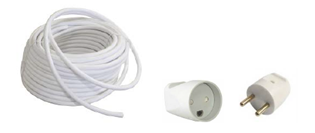
\includegraphics[scale=1]{Billeder/ledning.png}
\end{center}
En elektriker sælger forlængerledninger efter mål. Ledningen koster 2 kroner per meter, og de to elektriske stik koster 40 kroner i alt. 
\end{opgavetekst}
\begin{delopgave}{10 point}{1}
	Indfør passende variable, og opstil en formel, som viser sammenhængen mellem en forlængerledningens længde og samlede pris.
\end{delopgave}
\begin{meretekst}
Et byggemarked sælger også forlængerledninger efter mål. Her er den samlede pris $p$ for en forlængerledning på $x$ meter bestemt ved sammenhængen
\begin{align*}
p(x) = 2.5x+25
\end{align*} 
\end{meretekst}
\begin{delopgave}{10 point}{2}
Hvor lang en forlængerledning skal man købe, for det er billigst at handle hos elektrikeren?
\end{delopgave}

\begin{opgavetekst}{Opgave 7}

\begin{figure}[H]
\centering
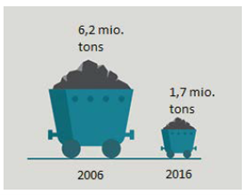
\includegraphics[scale=1]{Billeder/kul.png}
\caption{Ørsteds kulforbrug}
\label{fig:kul}
\end{figure}

På Fig. \ref{fig:kul} fremgår Ørsted A/S's (tidl. DONG Energy) anvendelse af kul til energiproduktion i årene 2006 og 2016. Udviklingen i perioden kan beskrives med en eksponentiel model $f$ med forskriften
\begin{align*}
f(x) = b \cdot a^x,
\end{align*}
hvor $x$ er antal år efter år 2006 og $f$ er mængden af kul, målt i mio. tons, der er anvendt til energiproduktion.
\end{opgavetekst}

\begin{delopgave}{10 point}{1}
Benyt Fig. \ref{fig:kul} til at bestemme tallene $a$ og $b$.
\end{delopgave}
\begin{delopgave}{5 point}{2}
Bestem halveringskonstanten for $f$.
\end{delopgave}
\begin{delopgave}{5 point}{3}
Hvad fortæller halveringskonstanten om udviklingen?
\end{delopgave}

\begin{delopgave}{10 point}{4}
Hvor stor vil mængden af kul være i 2023 i følge modellen, hvis udviklingen fortsætter?
\end{delopgave}

\begin{opgavetekst}{Opgave 8}
\begin{center}
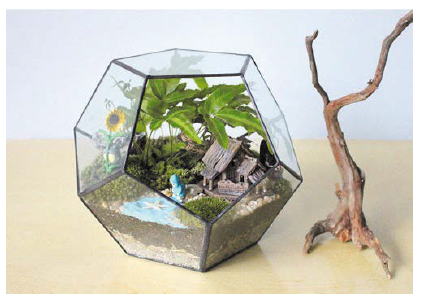
\includegraphics[scale=1]{Billeder/drivhus1}
\end{center}
Et dekorativt miniaturedrivhus er bygget af femkantede sideflader, hvis sidelængder $x$ alle er ens. Rumfanget af drivhuset kan med god tilnærmelse bestemmes ved udtrykket
\begin{align*}
f(x) = 0.00766 \cdot x^3,
\end{align*}
hvor $x$ er sidelængden af femkanterne målt i cm og $f(x)$ er rumfanget målt i liter. 
\end{opgavetekst}
\begin{delopgave}{5 point}{1}
Bestem rumfanget af et miniaturedrivhus med sidelængde $10$cm.
\end{delopgave}
\begin{delopgave}{5 point}{2}
Bestem sidelængden af et miniaturedrivhus med rumfanget 25L.
\end{delopgave}

\begin{meretekst}
\begin{center}
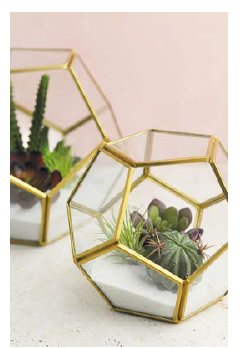
\includegraphics[scale=1]{Billeder/drivhus2}
\end{center}
I stedet for ét stort miniaturedrivhus kan vi få to mindre miniaturedrivhuse. Det oplyses, at sidelængden $x$ i det store drivhus er $25\%$ større end i de to små drivhuse. 
\end{meretekst}
\begin{delopgave}{10 point}{3}
	Hvor mange procent er rumfanget af det store drivhus større end rumfanget af det lille 			drivhus?
\end{delopgave}

\begin{opgavetekst}{Opgave 9}
\begin{center}
\includegraphics[width = 0.7\textwidth]{Billeder/newborn}
\end{center}

\begin{table}[H]
\centering
\begin{tabular}{c|c|c|c|c|c|c|c|c|c|c|c}
$x$ & 0 & 1 & 2 & 3 & 4 & 5 & 6 & 7 & 8 & 9 \\ \hline
 $y$ & 67.1 & 65.304 & 63.9 & 64.5 & 64.6 & 64.2 & 64.9 &64.1 & 65.0 & 62.8 
\end{tabular}
\caption{Antal levendefødte i Danmark i årene 2000-2009}
\label{tab:fodsel}
\end{table}
Af Tab. \ref{tab:fodsel} ses antallet af levendefødte $(y)$ i tusinder i årene $2000-2009$ $(x)$. 
\end{opgavetekst}
\begin{delopgave}{10 point}{1}
	Lav lineær og eksponentiel regression på datasættet fra Tab. \ref{tab:fodsel}. 
\end{delopgave}
\begin{delopgave}{10 point}{2}
	Lav residualanalyse på de to regressionsmodeller og afgør, hvilken af modellerne der er bedst.
\end{delopgave}
\begin{delopgave}{5 point}{3}
	Brug den bedste af de to modeller til at bestemme, hvor mange der fødes i 2010.
\end{delopgave}
\begin{delopgave}{5 point}{4}
	Afgør, hvornår din valgte model fortæller, at der fødes 60.000 levendefødte børn om året. 
\end{delopgave}
\end{document}



